% ============================================================
% Question Bank: ch04-03 Expanding Expressions with the Distributive Property
% Topic Title: Expanding Expressions with the Distributive Property
% CCSS: 7.EE.A.1
% Questions: 30 (18 MC + 7 SA + 5 Graphical)
% ============================================================

% --- Multiple Choice Questions (18) ---

\begin{practiceQuestion}{4-3-q01}{mc}
\begin{questionText}
Expand $3(x + 4)$.
\end{questionText}
\choiceA{$3x + 4$}
\choiceB{$3x + 12$}
\choiceC{$3x + 7$}
\choiceD{$12x$}
\correctAnswer{B}
\explanation{Multiply $3$ by each term: $3 \times x = 3x$ and $3 \times 4 = 12$. Result: $3x + 12$.}
\end{practiceQuestion}

\begin{practiceQuestion}{4-3-q02}{mc}
\begin{questionText}
Expand $5(2a - 3)$.
\end{questionText}
\choiceA{$10a - 3$}
\choiceB{$7a - 3$}
\choiceC{$10a - 15$}
\choiceD{$10a + 15$}
\correctAnswer{C}
\explanation{$5 \times 2a = 10a$ and $5 \times (-3) = -15$. Result: $10a - 15$.}
\end{practiceQuestion}

\begin{practiceQuestion}{4-3-q03}{mc}
\begin{questionText}
Expand $-2(3x + 7)$.
\end{questionText}
\choiceA{$-6x + 7$}
\choiceB{$-6x - 14$}
\choiceC{$-6x + 14$}
\choiceD{$6x - 14$}
\correctAnswer{B}
\explanation{$-2 \times 3x = -6x$ and $-2 \times 7 = -14$. Result: $-6x - 14$.}
\end{practiceQuestion}

\begin{practiceQuestion}{4-3-q04}{mc}
\begin{questionText}
Expand $-4(2y - 5)$.
\end{questionText}
\choiceA{$-8y - 20$}
\choiceB{$-8y - 5$}
\choiceC{$-8y + 20$}
\choiceD{$8y + 20$}
\correctAnswer{C}
\explanation{$-4 \times 2y = -8y$ and $-4 \times (-5) = +20$. A negative times a negative is positive. Result: $-8y + 20$.}
\end{practiceQuestion}

\begin{practiceQuestion}{4-3-q05}{mc}
\begin{questionText}
Which expression is equivalent to $6(n + 2)$?
\end{questionText}
\choiceA{$6n + 2$}
\choiceB{$6n + 8$}
\choiceC{$6n + 12$}
\choiceD{$8n$}
\correctAnswer{C}
\explanation{Distribute $6$: $6 \times n = 6n$ and $6 \times 2 = 12$. Result: $6n + 12$.}
\end{practiceQuestion}

\begin{practiceQuestion}{4-3-q06}{mc}
\begin{questionText}
Expand $\frac{1}{2}(8x - 6)$.
\end{questionText}
\choiceA{$4x - 6$}
\choiceB{$8x - 3$}
\choiceC{$4x - 3$}
\choiceD{$4x + 3$}
\correctAnswer{C}
\explanation{$\frac{1}{2} \times 8x = 4x$ and $\frac{1}{2} \times (-6) = -3$. Result: $4x - 3$.}
\end{practiceQuestion}

\begin{practiceQuestion}{4-3-q07}{mc}
\begin{questionText}
A student expands $-3(x - 4)$ and writes $-3x - 12$. What mistake did the student make?
\end{questionText}
\choiceA{Forgot to distribute to the second term}
\choiceB{Did not change the sign when multiplying $-3 \times (-4)$}
\choiceC{Multiplied only the first term}
\choiceD{Added instead of multiplying}
\correctAnswer{B}
\explanation{$-3 \times (-4)$ should equal $+12$, not $-12$. The correct expansion is $-3x + 12$.}
\end{practiceQuestion}

\begin{practiceQuestion}{4-3-q08}{mc}
\begin{questionText}
Expand and simplify $2(x + 3) + 5$.
\end{questionText}
\choiceA{$2x + 8$}
\choiceB{$2x + 11$}
\choiceC{$2x + 10$}
\choiceD{$7x + 3$}
\correctAnswer{B}
\explanation{Expand: $2x + 6$. Add $5$: $2x + 6 + 5 = 2x + 11$.}
\end{practiceQuestion}

\begin{practiceQuestion}{4-3-q09}{mc}
\begin{questionText}
Expand and simplify $4(2x + 1) + 3x$.
\end{questionText}
\choiceA{$11x + 1$}
\choiceB{$8x + 4$}
\choiceC{$11x + 4$}
\choiceD{$5x + 4$}
\correctAnswer{C}
\explanation{Expand: $8x + 4$. Add $3x$: $8x + 4 + 3x = 11x + 4$.}
\end{practiceQuestion}

\begin{practiceQuestion}{4-3-q10}{mc}
\begin{questionText}
Expand $-1(5a - 9)$.
\end{questionText}
\choiceA{$-5a + 9$}
\choiceB{$-5a - 9$}
\choiceC{$5a + 9$}
\choiceD{$5a - 9$}
\correctAnswer{A}
\explanation{$-1 \times 5a = -5a$ and $-1 \times (-9) = +9$. Result: $-5a + 9$. Multiplying by $-1$ flips the sign of every term.}
\end{practiceQuestion}

\begin{practiceQuestion}{4-3-q11}{mc}
\begin{questionText}
Expand and simplify $3(x - 2) + 2(x + 4)$.
\end{questionText}
\choiceA{$5x + 2$}
\choiceB{$5x - 2$}
\choiceC{$5x + 14$}
\choiceD{$x + 2$}
\correctAnswer{A}
\explanation{Expand each: $3x - 6 + 2x + 8$. Combine: $(3x + 2x) + (-6 + 8) = 5x + 2$.}
\end{practiceQuestion}

\begin{practiceQuestion}{4-3-q12}{mc}
\begin{questionText}
Expand $\frac{2}{3}(9x + 6)$.
\end{questionText}
\choiceA{$6x + 6$}
\choiceB{$6x + 4$}
\choiceC{$3x + 4$}
\choiceD{$18x + 4$}
\correctAnswer{B}
\explanation{$\frac{2}{3} \times 9x = 6x$ and $\frac{2}{3} \times 6 = 4$. Result: $6x + 4$.}
\end{practiceQuestion}

\begin{practiceQuestion}{4-3-q13}{mc}
\begin{questionText}
Expand and simplify $-2(3x + 1) + 4(x - 3)$.
\end{questionText}
\choiceA{$-2x - 14$}
\choiceB{$-2x + 14$}
\choiceC{$2x - 14$}
\choiceD{$-2x - 10$}
\correctAnswer{A}
\explanation{Expand: $-6x - 2 + 4x - 12$. Combine: $(-6x + 4x) + (-2 - 12) = -2x - 14$.}
\end{practiceQuestion}

\begin{practiceQuestion}{4-3-q14}{mc}
\begin{questionText}
Which expression is equivalent to $7(a - 3) - 2a$?
\end{questionText}
\choiceA{$5a - 3$}
\choiceB{$5a + 21$}
\choiceC{$9a - 21$}
\choiceD{$5a - 21$}
\correctAnswer{D}
\explanation{Expand: $7a - 21$. Subtract $2a$: $7a - 21 - 2a = 5a - 21$.}
\end{practiceQuestion}

\begin{practiceQuestion}{4-3-q15}{mc}
\begin{questionText}
Expand $-5(x + 2)$.
\end{questionText}
\choiceA{$-5x + 10$}
\choiceB{$-5x + 2$}
\choiceC{$-5x - 10$}
\choiceD{$5x - 10$}
\correctAnswer{C}
\explanation{$-5 \times x = -5x$ and $-5 \times 2 = -10$. Result: $-5x - 10$.}
\end{practiceQuestion}

\begin{practiceQuestion}{4-3-q16}{mc}
\begin{questionText}
Expand and simplify $2(4n - 3) - (n + 1)$.
\end{questionText}
\choiceA{$7n - 7$}
\choiceB{$9n - 7$}
\choiceC{$7n - 5$}
\choiceD{$9n - 4$}
\correctAnswer{A}
\explanation{Expand: $8n - 6 - n - 1$. Combine: $(8n - n) + (-6 - 1) = 7n - 7$.}
\end{practiceQuestion}

\begin{practiceQuestion}{4-3-q17}{mc}
\begin{questionText}
Expand $0.5(4x + 10)$.
\end{questionText}
\choiceA{$4.5x + 10.5$}
\choiceB{$2x + 5$}
\choiceC{$2x + 10$}
\choiceD{$4x + 5$}
\correctAnswer{B}
\explanation{$0.5 \times 4x = 2x$ and $0.5 \times 10 = 5$. Result: $2x + 5$.}
\end{practiceQuestion}

\begin{practiceQuestion}{4-3-q18}{mc}
\begin{questionText}
Which shows the correct expansion of $-3(2x - 4y + 1)$?
\end{questionText}
\choiceA{$-6x + 12y - 3$}
\choiceB{$-6x - 12y - 3$}
\choiceC{$-6x + 12y + 3$}
\choiceD{$-6x - 12y + 1$}
\correctAnswer{A}
\explanation{$-3 \times 2x = -6x$, $-3 \times (-4y) = +12y$, and $-3 \times 1 = -3$. Result: $-6x + 12y - 3$.}
\end{practiceQuestion}

% --- Short Answer Questions (7) ---

\begin{practiceQuestion}{4-3-q19}{sa}
\begin{questionText}
Expand $-6(2m - 5)$.
\end{questionText}
\correctAnswer{$-12m + 30$}
\explanation{$-6 \times 2m = -12m$ and $-6 \times (-5) = +30$. Result: $-12m + 30$.}
\end{practiceQuestion}

\begin{practiceQuestion}{4-3-q20}{sa}
\begin{questionText}
Expand and simplify $3(2x + 4) - 5x$.
\end{questionText}
\correctAnswer{$x + 12$}
\explanation{Expand: $6x + 12$. Subtract $5x$: $6x + 12 - 5x = x + 12$.}
\end{practiceQuestion}

\begin{practiceQuestion}{4-3-q21}{sa}
\begin{questionText}
Expand $\frac{3}{4}(8a - 12)$.
\end{questionText}
\correctAnswer{$6a - 9$}
\explanation{$\frac{3}{4} \times 8a = 6a$ and $\frac{3}{4} \times (-12) = -9$. Result: $6a - 9$.}
\end{practiceQuestion}

\begin{practiceQuestion}{4-3-q22}{sa}
\begin{questionText}
Expand and simplify $-2(x + 6) + 3(2x - 1)$.
\end{questionText}
\correctAnswer{$4x - 15$}
\explanation{Expand: $-2x - 12 + 6x - 3$. Combine: $(-2x + 6x) + (-12 - 3) = 4x - 15$.}
\end{practiceQuestion}

\begin{practiceQuestion}{4-3-q23}{sa}
\begin{questionText}
Expand and simplify $5(n - 3) - 2(n - 3)$.
\end{questionText}
\correctAnswer{$3n - 9$ or $3(n - 3)$}
\explanation{Expand: $5n - 15 - 2n + 6$. Combine: $(5n - 2n) + (-15 + 6) = 3n - 9$.}
\end{practiceQuestion}

\begin{practiceQuestion}{4-3-q24}{sa}
\begin{questionText}
A rectangular room has length $(2x + 3)$ feet and width $5$ feet. Write and expand an expression for its area.
\end{questionText}
\correctAnswer{$10x + 15$ square feet}
\explanation{Area $= 5(2x + 3) = 10x + 15$ square feet.}
\end{practiceQuestion}

\begin{practiceQuestion}{4-3-q25}{sa}
\begin{questionText}
Expand and simplify $-4(a - 2) + 3(a + 5) - 7$.
\end{questionText}
\correctAnswer{$-a + 16$}
\explanation{Expand: $-4a + 8 + 3a + 15 - 7$. Combine: $(-4a + 3a) + (8 + 15 - 7) = -a + 16$.}
\end{practiceQuestion}

% --- Graphical Questions (3 GMC + 2 GSA) ---

\begin{practiceQuestion}{4-3-q26}{gmc}
\begin{questionText}
The area model below represents a product. Which expression does it show?

\begin{center}
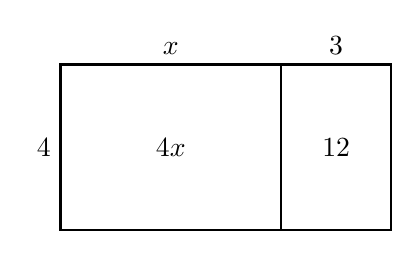
\begin{tikzpicture}[scale=0.7]
  % Outer rectangle
  \draw[thick] (0,0) rectangle (6,3);
  % Dividing line
  \draw[thick] (4,0) -- (4,3);
  % Labels
  \node[left] at (0,1.5) {$4$};
  \node[above] at (2,3) {$x$};
  \node[above] at (5,3) {$3$};
  % Inside labels
  \node at (2,1.5) {$4x$};
  \node at (5,1.5) {$12$};
\end{tikzpicture}
\end{center}
\end{questionText}
\choiceA{$4(x + 3) = 4x + 12$}
\choiceB{$4(x + 3) = 4x + 3$}
\choiceC{$3(x + 4) = 3x + 12$}
\choiceD{$(x + 3)(x + 4) = x^2 + 12$}
\correctAnswer{A}
\explanation{The height is $4$ and the width is split into $x$ and $3$. Multiply: $4 \times x = 4x$ and $4 \times 3 = 12$. So $4(x + 3) = 4x + 12$.}
\end{practiceQuestion}

\begin{practiceQuestion}{4-3-q27}{gmc}
\begin{questionText}
The area model shows a rectangle split into two parts. What is the expanded form?

\begin{center}
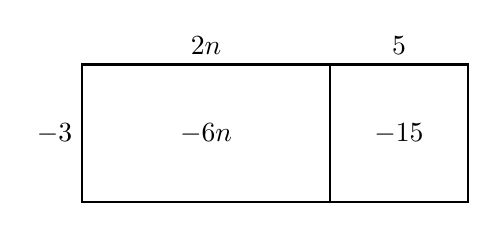
\begin{tikzpicture}[scale=0.7]
  \draw[thick] (0,0) rectangle (7,2.5);
  \draw[thick] (4.5,0) -- (4.5,2.5);
  \node[left] at (0,1.25) {$-3$};
  \node[above] at (2.25,2.5) {$2n$};
  \node[above] at (5.75,2.5) {$5$};
  \node at (2.25,1.25) {$-6n$};
  \node at (5.75,1.25) {$-15$};
\end{tikzpicture}
\end{center}
\end{questionText}
\choiceA{$-3(2n + 5) = -6n + 15$}
\choiceB{$-3(2n + 5) = -6n - 15$}
\choiceC{$-3(2n - 5) = -6n - 15$}
\choiceD{$3(2n + 5) = 6n + 15$}
\correctAnswer{B}
\explanation{The height is $-3$ and the width splits into $2n$ and $5$. Products: $-3 \times 2n = -6n$ and $-3 \times 5 = -15$. So $-3(2n + 5) = -6n - 15$.}
\end{practiceQuestion}

\begin{practiceQuestion}{4-3-q28}{gmc}
\begin{questionText}
Three friends each receive the same gift bag containing $x$ stickers and $4$ erasers. The diagram below represents the total items.

\begin{center}
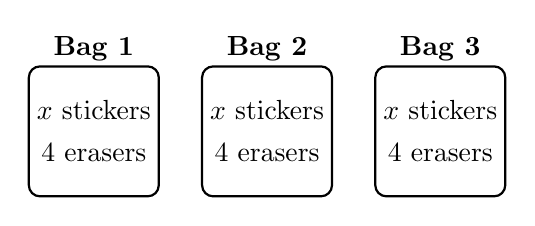
\begin{tikzpicture}[scale=0.55]
  % Bag 1
  \draw[thick, rounded corners] (0,0) rectangle (3,3);
  \node[font=\bfseries] at (1.5,3.4) {Bag 1};
  \node at (1.5,2) {$x$ stickers};
  \node at (1.5,1) {$4$ erasers};
  % Bag 2
  \draw[thick, rounded corners] (4,0) rectangle (7,3);
  \node[font=\bfseries] at (5.5,3.4) {Bag 2};
  \node at (5.5,2) {$x$ stickers};
  \node at (5.5,1) {$4$ erasers};
  % Bag 3
  \draw[thick, rounded corners] (8,0) rectangle (11,3);
  \node[font=\bfseries] at (9.5,3.4) {Bag 3};
  \node at (9.5,2) {$x$ stickers};
  \node at (9.5,1) {$4$ erasers};
\end{tikzpicture}
\end{center}

Which expression represents the total number of items?
\end{questionText}
\choiceA{$3x + 4$}
\choiceB{$x + 12$}
\choiceC{$3(x + 4) = 3x + 12$}
\choiceD{$3x + 4 + 4 + 4 = 3x + 4$}
\correctAnswer{C}
\explanation{Each bag has $x + 4$ items. With $3$ bags: $3(x + 4) = 3x + 12$ total items.}
\end{practiceQuestion}

\begin{practiceQuestion}{4-3-q29}{gsa}
\begin{questionText}
Use the area model to expand $5(3x + 2)$. Fill in the missing values and write the expanded expression.

\begin{center}
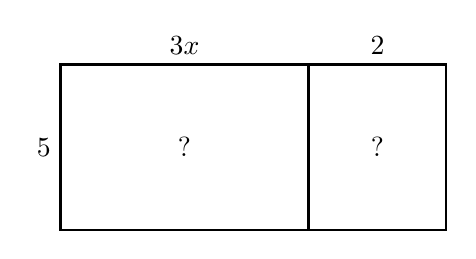
\begin{tikzpicture}[scale=0.7]
  \draw[thick] (0,0) rectangle (7,3);
  \draw[thick] (4.5,0) -- (4.5,3);
  \node[left] at (0,1.5) {$5$};
  \node[above] at (2.25,3) {$3x$};
  \node[above] at (5.75,3) {$2$};
  \node at (2.25,1.5) {?};
  \node at (5.75,1.5) {?};
\end{tikzpicture}
\end{center}
\end{questionText}
\correctAnswer{$15x + 10$}
\explanation{The left section: $5 \times 3x = 15x$. The right section: $5 \times 2 = 10$. Expanded: $5(3x + 2) = 15x + 10$.}
\end{practiceQuestion}

\begin{practiceQuestion}{4-3-q30}{gsa}
\begin{questionText}
The diagram shows two rectangles placed side by side. Write a simplified expression for the total area.

\begin{center}
\begin{tikzpicture}[scale=0.7]
  % Rectangle 1
  \draw[thick, fill=funBlue!10] (0,0) rectangle (4,3);
  \node[below] at (2,0) {$2x + 1$};
  \node[left] at (0,1.5) {$3$};
  \node at (2,1.5) {Area $= ?$};
  % Rectangle 2
  \draw[thick, fill=funOrange!10] (5,0) rectangle (8.5,3);
  \node[below] at (6.75,0) {$x - 2$};
  \node[right] at (8.5,1.5) {$3$};
  \node at (6.75,1.5) {Area $= ?$};
\end{tikzpicture}
\end{center}
\end{questionText}
\correctAnswer{$9x - 3$}
\explanation{Area 1: $3(2x + 1) = 6x + 3$. Area 2: $3(x - 2) = 3x - 6$. Total: $(6x + 3) + (3x - 6) = 9x - 3$.}
\end{practiceQuestion}
